\begin{figure}[htbp]
\centering
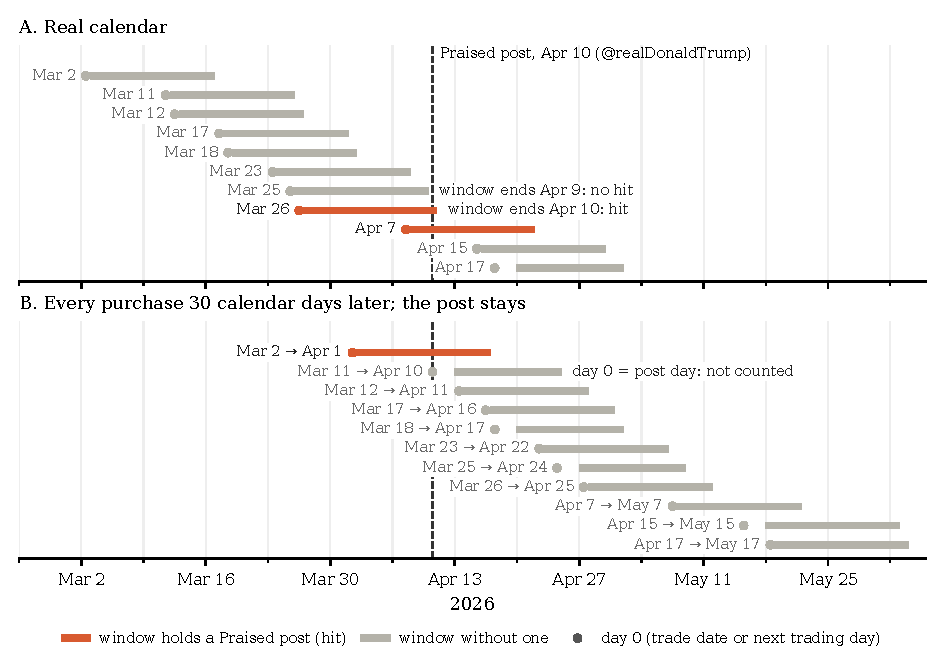
\includegraphics[width=\linewidth]{fig_palantir.pdf}
\caption{Palantir: the window, the hits and the shifted world with the smallest shift}
\label{fig:palantir}
\par\medskip
\begin{minipage}{\linewidth}\footnotesize\textit{Note:} Each row is one purchase of Palantir (PLTR) with a trade date between March 1 and April 20, 2026, the same eleven purchases in both panels: dot = day 0, bar = trading days 1 to 10. Labels give the disclosed trade date and, in panel B, the calendar date to which the shift moves it. The dashed line is the post of April 10, 2026 on @realDonaldTrump (sentiment 1.0), one of the two Praised direct mentions of Palantir in the sample; the other, a @WhiteHouse post of July 15, 2026, lies outside the figure. In the real calendar the purchases of March 26 and April 7 are hits, whereas the window of March 25 ends on April 9. Panel B shows the world with the smallest shift, 30 days, which comes first by rule and was not chosen by its outcome. There the purchase of March 2 moves to April 1 and becomes a hit with the same post, the purchase of March 11 moves to April 10, where the post falls on day 0 and does not count, and the real hits move past the post. The same world has a second Palantir hit outside the figure, a purchase of June 3 moved to July 3, with the post of July 15. Across the 499 shifted worlds Palantir has on average 3.08 purchases followed by a Praised post, against 2 in the real calendar, and 478 of the 499 worlds have at least one.\end{minipage}
\end{figure}
